\subsection{Historia}
La protagonista es una abuelita octogenaria que vive plácidamente en su casita situada en una agradable zona residencial. Todo iba de maravilla hasta que se ve invadida por terribles zombies. Es entonces cuando, lo que parecía una inocente y respetable abuela (como la que podemos tener todos nosotros), decide arrastrar con ella a todos los engendros que pueda de camino al infierno. ¿Será nuestra abuelita un digno rival para el apocalipsis que se presenta?.\\

¡Ayúdala en su periplo por el apocalipsis!

\subsection{La abuelita}
Debajo de esa bata y ese camisón (no le dio tiempo de cambiarse cuando la atacaron los zombies) se esconde una bestia iracunda. Su descanso se ha visto interrumpido y esos putrefactos zombies maleducados deben pagar por ello.

\begin{center}
	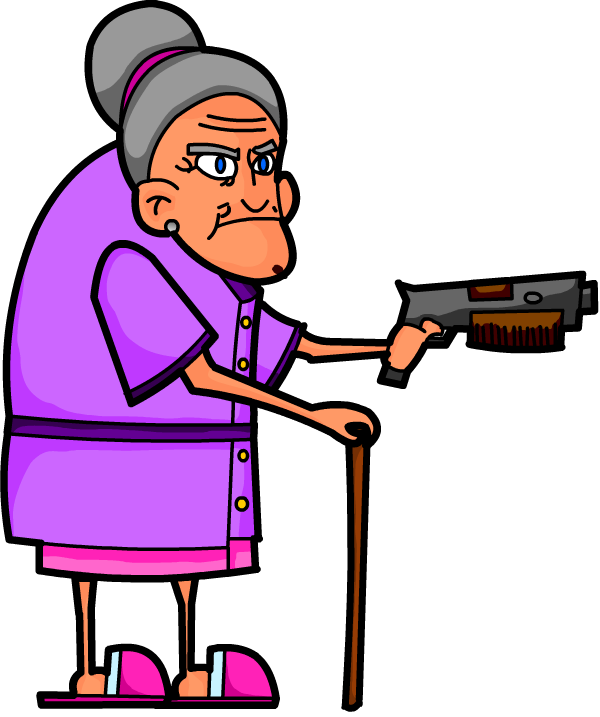
\includegraphics[scale=0.2]{granny.png}
\end{center}

\subsection{La horda}
¡Cuidado con los zombies! Te encontrarás con distintos tipos a lo largo del juego y debes trazar la mejor estrategia posible para enfrentarte a cada uno de ellos ya que tienen habilidades distintas:

\begin{center}
	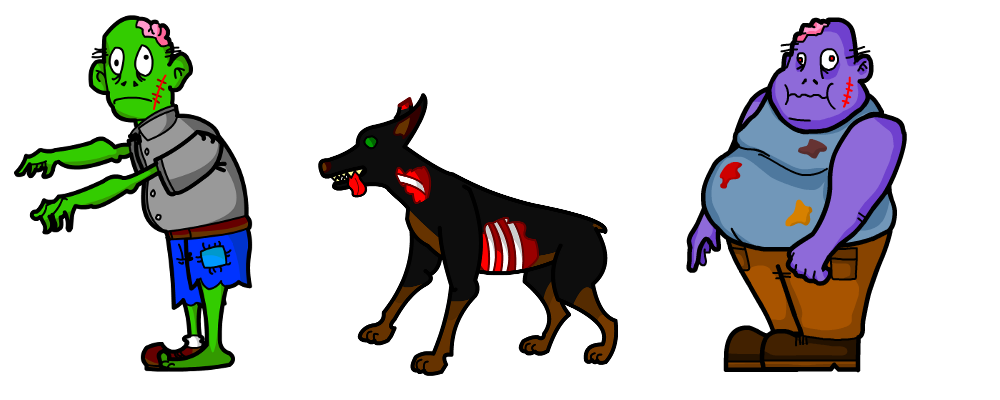
\includegraphics[scale=0.35]{enemigos.png}
\end{center}

\begin{itemize}
	\item \emph{Zombie genérico:} El clásico enemigo que se repite en todos los juegos y nosotros no tenemos la decencia siquiera de cambiarlo de color. Se moverá torpemente persiguiendo a ala abuela y si te toca serñas dañando. Es sencillo de eliminar.
	\item \emph{Perro zombie rabioso:} Con una clara inspiración de la saga Resident Evil (¡Shhhhh que nos pediran derechos de autor!) llega este sabueso asesino. Su velocidad pondrá nervioso a más de uno así que ten cuidado, no podrás huir.
	\item \emph{Zombie gordo:} En otra vida fue cliente honorífico de cierta cadena de hamburgueserías americana y ahora no para de devolver lo que un día zampó. Es cierto que se mueve con extrema lentitud pero sus vómitos corrosivos (aparte que dan un asco tremendo) pueden acabar contigo en un plis plas.
\end{itemize}

\paragraph{}
¡Cuidado! Puede que en la aventura de la abuelita te topes con otros enemigos mucho más terribles que los anteriores.

\subsection{Los preciados items}
¡La abuelita no está sóla! Cuenta con diversos objetos que la ayudarán en su objetivo. ¡Se inteligente, audaz y encuéntralos todos para sobrevivir!

\begin{center}
 	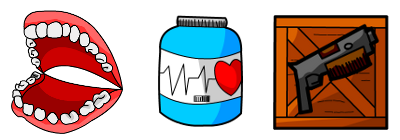
\includegraphics[scale=0.6]{items.png}
\end{center}

\begin{itemize}
	\item \emph{Dentaduras postizas:} ¿Qué sería de una abuelita sin sus dentaduras postizas? Estarán en las zonas más inaccesibles de cada nivel pero obtendrás puntos al recogerlas y si consigues 10, ganarás una vida.
	\item \emph{Pastillas para la tensión:} Los zombies pueden hacer mella en una abuelita fácilmente así que recogiendo tus queridas pastillas recuperarás parte de tu energía.
	\item \emph{Munición de la escopeta:} Decidida a acabar con todos los zombies, la abuela recoge la escopeta de su difunto marido. ¡No te apresures disparando! La muninción es limitada y la recuperarás recogiendo estos objetos.
\end{itemize}
